\documentclass[10pt,a4paper]{article}
\usepackage[utf8]{inputenc}
\usepackage{tikz}
\usepackage{pgfplots, pgfplotstable}
\usepackage{ae}
\usepackage[brazil]{babel}
\usepackage[vmargin=2cm,hmargin=2cm,columnsep=0.75cm]{geometry}
\usepackage{float,nonfloat}
\usepackage{graphicx,color}
\usepackage{subcaption}
\usepackage{amsmath}
\usepackage{verbatim}
\usepackage{booktabs}
\usepackage{multirow}

\makeatletter
\let\@institution\empty
\def\institution#1{\def\@institution{#1}}
\renewcommand{\maketitle}{
    \begin{center}
        {\Large\bfseries\@title\par\medskip}
        {\large
            \begin{tabular}[t]{c}%
                \@author
        \end{tabular}\par\medskip}
        {\itshape\@institution\par}
        {\itshape\@date\par}
\end{center}}
\makeatother

\newcommand{\pixel}{\textit{pixel} }
\newcommand{\pixels}{\textit{pixels} }
\newcommand{\kernel}{\textit{kernel} }
\newcommand{\kernels}{\textit{kernels} }

\begin{document}
% ============================================================================

\title{MC920: Introdução ao Processamento de Imagem Digital\\Tarefa 9}
\author{
    \begin{minipage}{6cm}
        \centering
        Martin Ichilevici de Oliveira\\
        RA 118077
    \end{minipage}
    \and
    \begin{minipage}{6cm}
        \centering
        Rafael Almeida Erthal Hermano\\
        RA 121286
    \end{minipage}
}
\institution{Instituto de Computação, Universidade Estadual de Campinas}
\date{\today}

\maketitle

% ============================================================================
\section{Transformada de Fourier aplicada a impressões digitais}
Neste trabalho, estudou-se a aplicação da Transformada de Fourier (FT) a impressões digitais, com o intuito de verificar se e possível utilizar a FT para caracterizar univocamente uma impressão digital.

Dada uma imagem de impressão digital, a subdividimos em blocos de em blocos $w \times w$, com uma sobreposição entre eles de $\frac{w}{2}\times\frac{w}{2}$, de forma a não perder a continuidade entre os blocos. Em seguida, aplicou-se a Transformada de Fourier, e transladou-se o o termo de frequência zero $(u_0, v_0)$ para o centro da imagem. Em seguida, determinou-se o ponto (frequência) com maior intensidade $(u_p, v_p)$, execetuando o centro. A distância euclidiana entre $(u_p, v_p)$ e $(u_0, v_0)$, expressa em (\ref{eq:dist}), é a frequência máxima $f_r$ da imagem, e corresponde ao número de cristas no bloco. Além disso, o ângulo entre estes dois pontos, $\theta_r$, é a orientação (perpendicular) das cristas na imagem.

\begin{equation}
    f_r = d = \sqrt{(u_p - u_0)^2 + (v_p - v_0)^2}
    \label{eq:dist}
\end{equation}

\section{Experimentos}
Adotamos $w=16$, de forma que cada bloco tinha uma sobreposição de 8 \pixels com seus vizinhos.

A tabela \ref{tab:ex} mostra alguns exemplos de blocos, o número de cristas (determinado visualmente), $f_r$ e $\theta_r$ calculados. Podemos observar que o método foi muito eficaz para determinar o número de cristas e a direção das mesmas em cada bloco.
\begin{table}[!ht]
    \caption{Exemplos de blocos e resultados obtidos}
    \label{tab:ex}
    \begin{tabular}{ccccc}
        \toprule
        Imagem & FFT & Cristas & $f_r$ & $\theta_r$ (rad)\\\midrule
        \fbox{
\includegraphics[width=32px,height=32px]{region16-03.png}} & \fbox{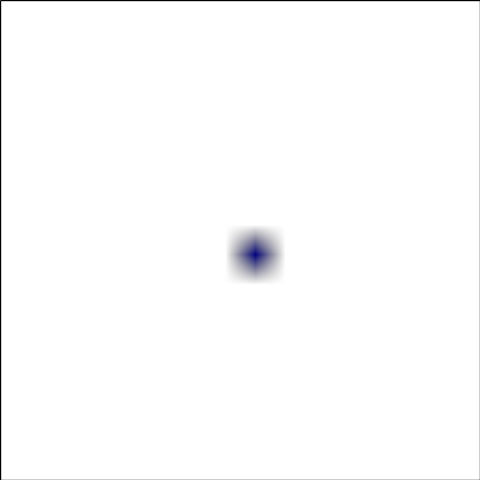
\includegraphics[width=32px,height=32px]{fft03.png}} & 0 & 0    & $\pi/2$\\
        \fbox{
\includegraphics[width=32px,height=32px]{region16-40.png}} & \fbox{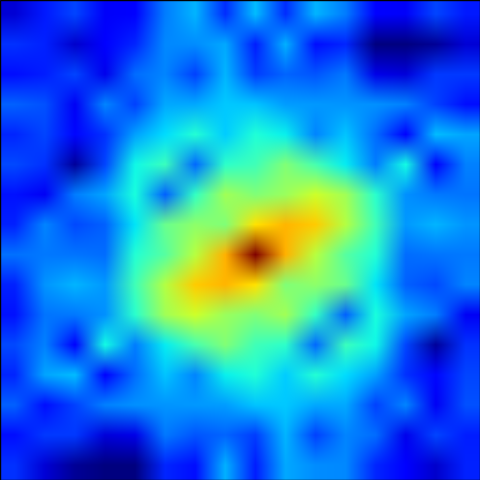
\includegraphics[width=32px,height=32px]{fft40.png}} & 1 & 1    & $\pi/2$\\
        \fbox{
\includegraphics[width=32px,height=32px]{region16-20.png}} & \fbox{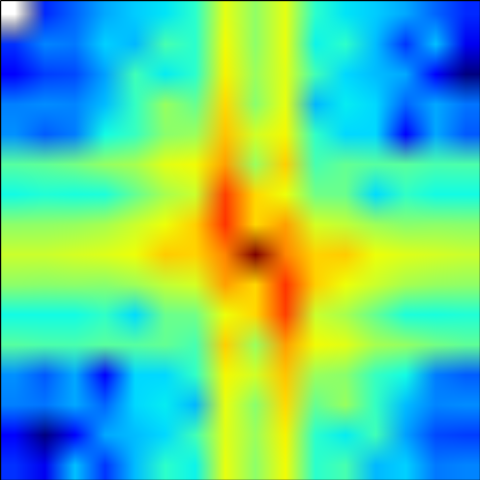
\includegraphics[width=32px,height=32px]{fft20.png}} & 2 & 1.41 & $\pi/4$\\
        \fbox{
\includegraphics[width=32px,height=32px]{region16-23.png}} & \fbox{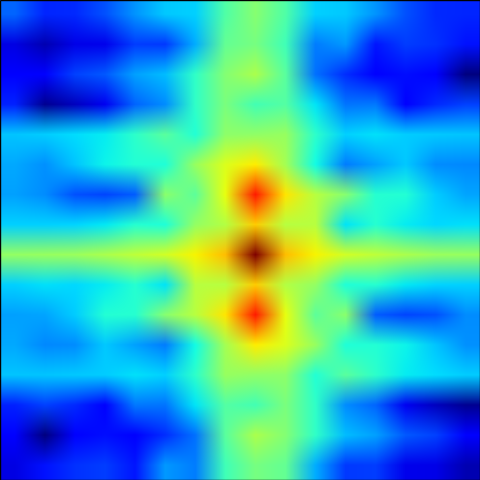
\includegraphics[width=32px,height=32px]{fft23.png}} & 2 & 2    & 0\\
        \fbox{
\includegraphics[width=32px,height=32px]{region16-26.png}} & \fbox{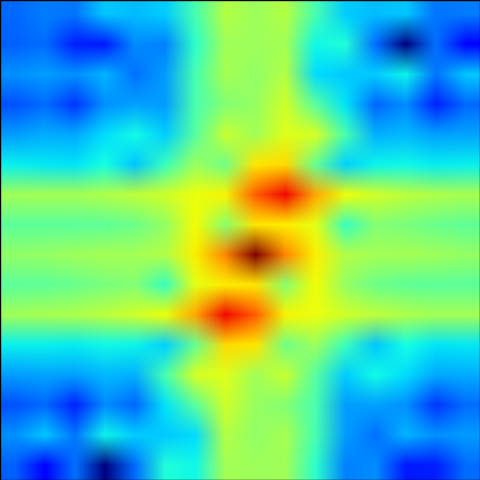
\includegraphics[width=32px,height=32px]{fft26.png}} & 2 & 2.24 & $-\pi/4$\\
        \fbox{
\includegraphics[width=32px,height=32px]{region16-30.png}} & \fbox{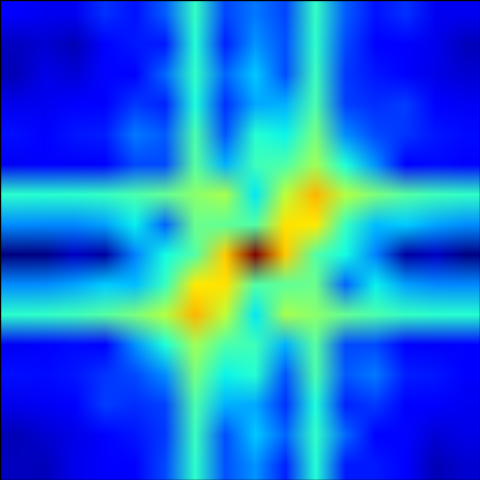
\includegraphics[width=32px,height=32px]{fft30.png}} & 3 & 2.83 & $-\pi/4$\\
        \bottomrule
     \end{tabular}
\end{table}

A Figura \ref{fig:line} mostra o valor de $f_r$ para uma única linha da impressão digital. Os blocos que a compõem estão expressos na Figura \ref{fig:line_attached} -- note que, como os blocos possuem uma sobreposição, esta imagem não é fluída, já que ela manteve os trechos duplicados de cada bloco. Podemos ver que não há grandes saltos na imagem, dada a técnica de sobreposição utilizada.

\begin{figure}
    \begin{subfigure}[!ht]{\textwidth}
    \centering
    \fbox{
\includegraphics[width=0.8\textwidth]{16_stitched.png}}
        \caption{Blocos de linha ligados.}
        \label{fig:line_attached}
    \end{subfigure}
    \\
    \begin{subfigure}[!ht]{0.45\textwidth}
        \begin{tikzpicture}
            \begin{axis}[xlabel=i, ylabel=d]
                \addplot file{line.txt};
            \end{axis}
        \end{tikzpicture}
        \caption{Frequência máxima na linha 16}
        \label{fig:line_freq}
    \end{subfigure}
    \caption{Dados para apenas uma linha da imagem}
    \label{fig:line}
\end{figure}

Por fim, a Figura \ref{fig:fingerprint_all} mostra o valor de $f_r$ para todos os blocos de algumas impressões digitais. É nítido que as distribuições são bem diferentes -- isto é um bom indicativo de que o método é capaz de distinguir diferentes impresões digitais.
\begin{figure}[!htb]
    \begin{subfigure}[ht]{0.45\textwidth}
    \centering
        \fbox{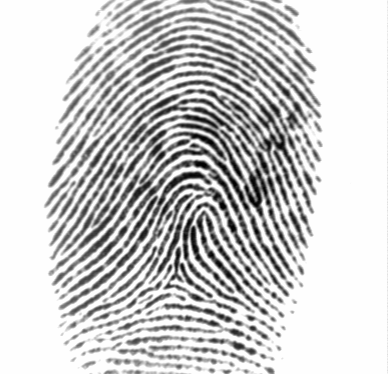
\includegraphics[width=0.8\columnwidth]{1_1.png}}
        \caption{Blocos de linha ligados.}
        \label{fig:fingerprint}
    \end{subfigure}
    \qquad
    \begin{subfigure}[ht]{0.45\textwidth}
        \begin{tikzpicture}
            \begin{axis}[xlabel=i, ylabel=j, zlabel=d]
                \addplot3[surf] file{all1.txt};
            \end{axis}
        \end{tikzpicture}
        \caption{$f_r$ para todos os blocos}
        \label{fig:fingerprint_all}
    \end{subfigure}
    \\
    \begin{subfigure}[ht]{0.45\textwidth}
    \centering
        \fbox{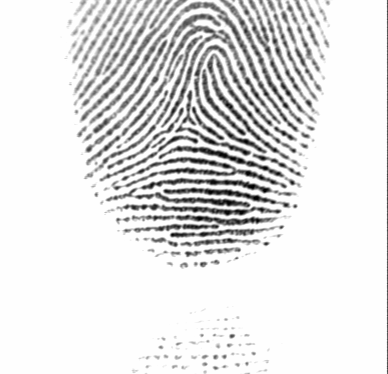
\includegraphics[width=0.8\columnwidth]{1_4.png}}
        \caption{Blocos de linha ligados.}
        \label{fig:fingerprint}
    \end{subfigure}
    \qquad
    \begin{subfigure}[ht]{0.45\textwidth}
        \begin{tikzpicture}
            \begin{axis}[xlabel=i, ylabel=j, zlabel=d]
                \addplot3[surf] file{all4.txt};
            \end{axis}
        \end{tikzpicture}
        \caption{$f_r$ para todos os blocos}
        \label{fig:fingerprint_all}
    \end{subfigure}
    \\
    \begin{subfigure}[ht]{0.45\textwidth}
    \centering
        \fbox{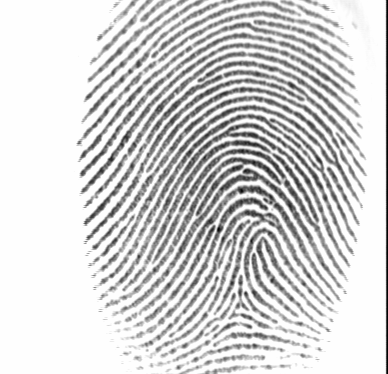
\includegraphics[width=0.8\columnwidth]{1_8.png}}
        \caption{Blocos de linha ligados.}
        \label{fig:fingerprint}
    \end{subfigure}
    \qquad
    \begin{subfigure}[ht]{0.45\textwidth}
        \begin{tikzpicture}
            \begin{axis}[xlabel=i, ylabel=j, zlabel=d]
                \addplot3[surf] file{all8.txt};
            \end{axis}
        \end{tikzpicture}
        \caption{$f_r$ para todos os blocos}
        \label{fig:fingerprint_all}
    \end{subfigure}
    \caption{Frequência máxima em cada sub-imagem}
    \label{fig:all}
\end{figure}

\end{document}
